\documentclass{report}
\usepackage[T1]{fontenc}
\usepackage{color}
\usepackage{amssymb}
\usepackage{amsmath}
\usepackage{eurosym}
\usepackage{graphicx}
\usepackage{textcomp}
\usepackage{listings}
\usepackage{epigraph}
\usepackage{setspace}
\usepackage[some]{background}
\usepackage{gensymb}
\usepackage{tikz}
\usepackage{fancyhdr}
\usepackage[margin=0.9in]{geometry}
\usepackage[english]{babel}
\lstdefinelanguage{scala}{
morekeywords={%
abstract,case,catch,class,def,do,else,extends,%
false,final,finally,for,forSome,if,implicit,import,lazy,%
match,new,null,object,override,package,private,protected,%
return,sealed,super,this,throw,trait,true,try,type,%
val,var,while,with,yield},
otherkeywords={=>,<-,<\%,<:,>:,\#,@},
sensitive=true,
morecomment=[l]{//},
morecomment=[n]{/*}{*/},
morestring=[b]",
morestring=[b]',
morestring=[b]"""
}[keywords,comments,strings]

\lstset{
float=hbp,
language=scala,
basicstyle=\ttfamily\small\color{colBasic},
upquote=true,
aboveskip={1.5\baselineskip},
columns=fullflexible,
showstringspaces=false,
extendedchars=true,
breaklines=true,
showtabs=false,
showspaces=false,
frame=trbl, 
tabsize=4,
numbers=left,
breakautoindent=true,
extendedchars=true,
showstringspaces=false,
identifierstyle=\ttfamily,
frameround=ffff,
captionpos=b,
xrightmargin=0cm,
xleftmargin=0cm,
backgroundcolor=\color{colBackground},
keywordstyle=\bf\color{colKeyword},
commentstyle=\color{colComment},
identifierstyle=\color{colIdent}, 
stringstyle=\color{colString},}\definecolor{colBasic}{rgb}{0.7,0.44,0.23}
\definecolor{colKeyword}{rgb}{0.58,0.15,0.5}
\definecolor{colBackground}{rgb}{0.15,0.15,0.15}
\definecolor{colComment}{rgb}{0.4,0.4,0.4}
\definecolor{colString}{rgb}{0.9,0.4,0}
\definecolor{colIdent}{rgb}{1,0.75,0.75}


\begin{document}
\renewcommand{\chaptername}{Chapter}
\renewcommand{\thechapter}{\Roman{chapter}}

\pagestyle{fancy}
%\usepackage{lmodern}
%\usepackage{xspace}
%\usepackage{hyperref}
%\usepackage{fancyhdr}

% header style
\pagestyle{fancy}
\renewcommand{\headrulewidth}{1pt}
\fancyhead[L]{February $12^{th}$ 2015}
\fancyhead[R]{\textbf{Reference :} model-checking.archi - Version 1}

% Redefine the plain page style
\fancypagestyle{plain}{%
  \fancyhf{}%
  \renewcommand{\headrulewidth}{1pt}
  \fancyhead[L]{February $12^{th}$ 2015}
  \fancyhead[R]{\textbf{Reference :} model-checking.archi - Version 1}
  \fancyfoot[C]{\thepage}
}

% title page
\definecolor{sup_strip_color}{rgb}{0.70,0.70,0.70}
\definecolor{inf_strip_color}{rgb}{0.00,0.00,0.00}

\DeclareFixedFont{\bigsf}{T1}{phv}{b}{n}{0.7cm}

\makeatletter                       
\def\printauthor{%                  
    {{\large \@author}}}              
\makeatother

\author{Zohour \textsc{Abouakil} ~\\ Sofia \textsc{Boutahar} ~\\ David \textsc{Courtinot} ~\\ Xiaowen \textsc{Ji} ~\\ Fabien \textsc{Sauce}}

\begin{titlepage}

\newgeometry{left=1cm,right=4cm,bottom=0cm}
\begin{tikzpicture}[overlay,remember picture]
% the black stripe with the title
\node[
  fill=inf_strip_color,
  anchor=north west,
  text width=\paperwidth,
  text height=2cm,
  text depth=2cm,
  inner xsep=1cm,
  font=\color{white}\bigsf 
  ] 
 at ([yshift=-2.5cm]current page.north west) (blackrect) {Architecture document - Version 1};
% the khaki stripe
\path[fill=sup_strip_color] 
  (blackrect.north west) rectangle ++(\paperwidth,2.5cm);
\end{tikzpicture}

\vspace*{4.5cm}

\noindent
\begin{minipage}{0.35\linewidth}
    \begin{flushright}
        \printauthor
    \end{flushright}
\end{minipage} \hspace{15pt}
%
\begin{minipage}{0.02\linewidth}
    \rule{1pt}{175pt}
\end{minipage} \hspace{-10pt}
%
\begin{minipage}{0.6\linewidth}
\vspace{5pt}
\newenvironment{test}{\begin{center}}{\end{center}}
\hspace{10pt}
\begin{minipage}{\linewidth} 
\textbf{Reference :} model-checking.archi ~\\
February $12^{th}$ 2015
\end{minipage}
\end{minipage}

\vspace{8cm}
\begin{minipage}{0.20\linewidth}
    \begin{flushright}
       
        \begin{tabular}{ll}
	 \textit{Signatures} & \\
			& \textbf{Project manager - Zohour \textsc{Abouakil} :} \\
            & \textbf{Quality responsible - David \textsc{Courtinot} :} \\
            & \textbf{Customers - David \textsc{Doose} - Julien \textsc{Brunel} :} \\
        \end{tabular}
    \end{flushright}
\end{minipage}

\end{titlepage}
\restoregeometry
\tableofcontents
\newgeometry{left=2.1cm,right=2.1cm}
\chapter{Context}

\section{Objectives and motivations}

\paragraph{}
\hspace{4mm}\textnormal{As everyone knows, embedded systems are most often critical systems and must be as robust as possible to avoid critical failures which could have dramatic consequences.
Hence, many researches are done in order to build tools that would help to ensure the good properties of an embedded system source code and compensate potential human
failure. The model checking, which consists in asserting properties on a model thanks to graph search algorithms (for example), is one of those fields that can be
applied to this matter. In this project, we are trying to build a model checker working on C++ code which takes the source code as an input and is transformed a few times
in various abstract representations to end with a graph model that we are able to send to a model checker.}

\section{Definitions}

\subsection{AST - Abstract Syntax Tree}

\paragraph{}
\hspace{4mm}\textnormal{The AST is an abstract (and low-level) representation of the code. It is a tree data-structure which describes the code in a purely syntactic point of view. As an example,
you can see below a simple C/C++ code and its AST representation. The AST is provided by the Clang API, which performs the first step of our
transformation chain.}

\begin{lstlisting}[language=java]
void fun(int &a) {
    ++a;
}

int main(int argc, char* argv[]) {
    int num = 10;
    if (num > 5)
        fun(num);
    
    return 0;
}
\end{lstlisting}
\begin{center}
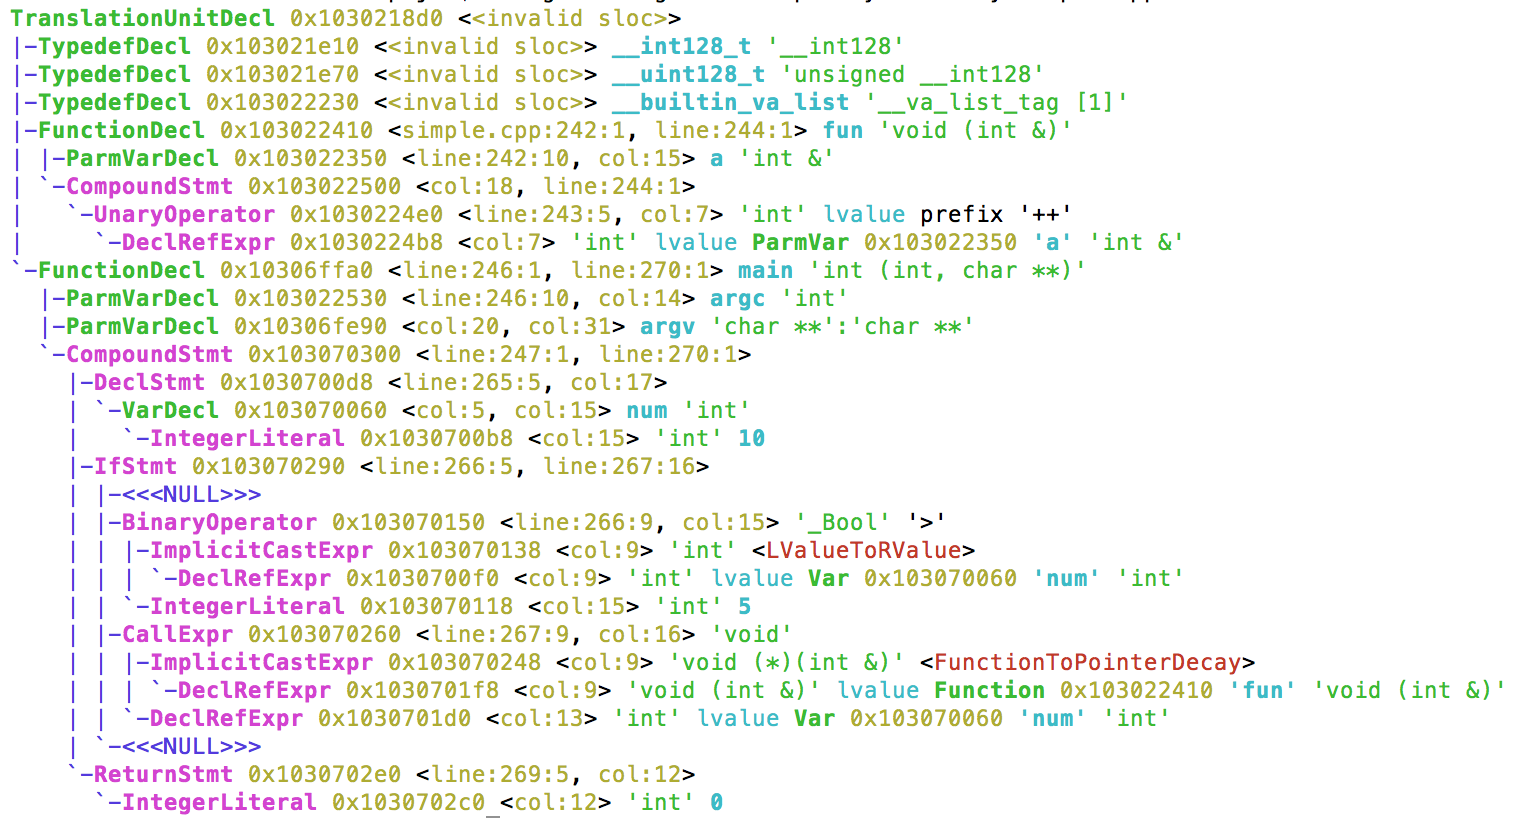
\includegraphics[scale=0.5]{data/ast.png}
~\\~\\Figure I.1 - The AST corresponding to the above code
\end{center}

\subsection{CFG - Control Flow Graph}

\paragraph{}
\hspace{4mm}\textnormal{The CFG is a graph representing all the possible execution paths (with some restrictions, for example
we won't create several nodes for a single expression even if in reality an expression should be a graph).
As an example, you can find below the CFG generated by a  do while statement in an if statement.}

\begin{center}
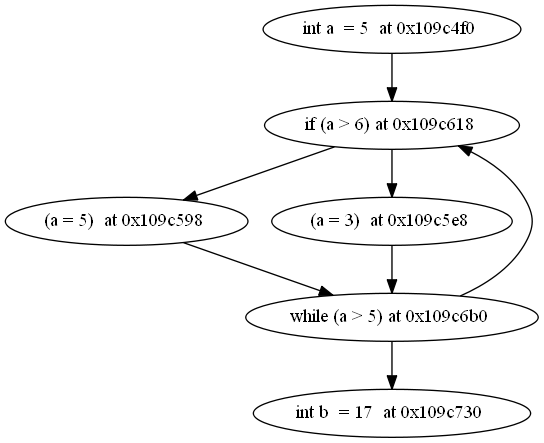
\includegraphics[scale=0.45]{data/doWhile.png}
~\\~\\Figure I.2 - An example of CFG
\end{center}

\subsection{CTL - Computation Tree Logic}

\paragraph{}
\hspace{4mm}\textnormal{CTL is a way of representing temporal logic expressions on a graph or a tree. For example, it can
express properties such as \textit{<< All the paths starting from every node verifies the predicate p >>}.}

\chapter{AST and CFG representations}

\paragraph{}
\hspace{4mm}\textnormal{After studying the Clang API, we came to the conclusion that the AST is a much more low-level representation of the program than the CFG. 
Indeed, the atom for a CFG is what is generally called a \textit{statement} whereas the simplest instruction
gives an AST representation composed of multiple nodes. We also found it difficult to handle the parsing and the linking of the graph nodes at the same time.
Thus, we have chosen to transform the AST into a series of higher-level objects than the original nodes, which will be converted
in nodes of the CFG.}

\begin{center}
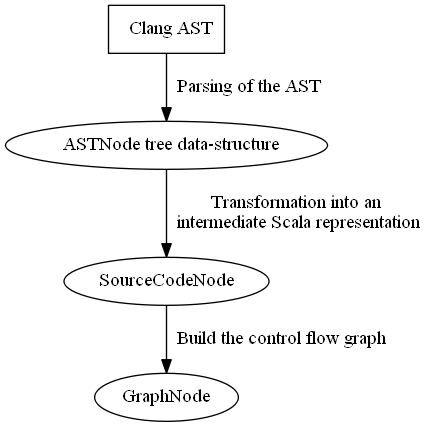
\includegraphics[scale=0.5]{data/transform_chain.png}
~\\~\\Figure II.1 - Transformation chain we are going to present
\end{center}

\section{Intermediate representation of the Clang AST}

\subsection{Parsing the Clang AST file}

\paragraph{}
\hspace{4mm}\textnormal{At first, we have considered using XML parsing libraries to parse the XML version of the Clang AST. However, 
this type of output is no longer supported by the newest versions of the Clang compiler and all the existing tools
provide partial support at best. Hence, we decided using the regular AST file and parse it line by line 
with a custom parser.}

\paragraph{}
\hspace{4mm}\textnormal{We have identified three main kinds of nodes in the AST. Each one is associated to a specific class which extends ASTNode :}

\vspace{1.5mm}
\begin{itemize}
\item nodes consisting in an type name, an id, a code pointer pointing the relevant lines of the code and some
metadata that depend on the type of the node. These are represented by the ConcreteASTNode class.\vspace{1mm}
\item < < <NULL> > > children, represented by the NullASTNode class.\vspace{1mm}
\item other kind of nodes, prior to class declaration for example. These are represented by OtherASTNode.\vspace{1mm}
\end{itemize}

\paragraph{}
\hspace{4mm}\textnormal{The file will be parsed and converted in a tree data-structure which nodes are of type ASTNode. The ASTNode objects
will then be converted in Stmt or Decl accordingly to the class hierarchy we present in the next part.}

\begin{center}
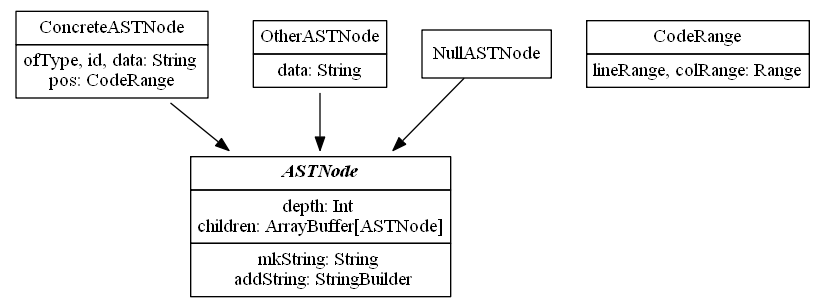
\includegraphics[scale=0.5]{data/AST_classes.png}
~\\~\\Figure II.2 - Class hierarchy for the output format of the ASTParser
\end{center}

\subsection{From ASTNode to SourceCodeNode}

\paragraph{}
\hspace{4mm}\textnormal{The SourceCodeNode class represents a tree data-structure which is still close enough to the AST 
but with a higher abstraction, and some removed low-level information.}

\subsubsection{Decl class hierarchy}

\paragraph{}
\hspace{4mm}\textnormal{For the Decl part,  which represents the different kinds of declarations in the code, we did not have too much trouble and just had to associate each high-level Clang Decl class to a Scala class extending
our Decl class, as it is shown in the previous figure.}

\subsubsection{Stmt part}

\paragraph{}
\hspace{4mm}\textnormal{Stmt is a Clang asbtraction of a statement in a program (any expression, any flow-control structure). As it was not presented as a priority by the client, we have decided to skip the C++ object oriented 
part in order to focus exclusively on the imperative part. Inspired by the Clang API, we came up
 with the following class diagram :}

\begin{center}
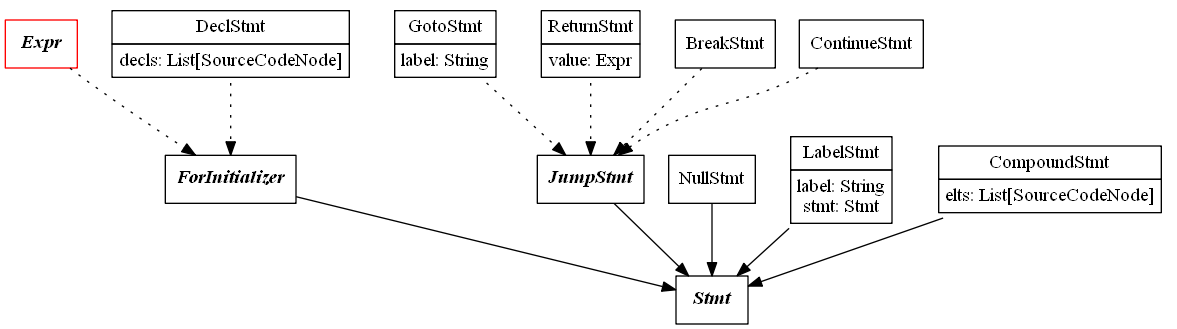
\includegraphics[scale=0.4]{data/basic_Stmt_classes.png}
~\\~\\Figure II.3 - Representation of the most classes statements
\end{center}

\begin{center}
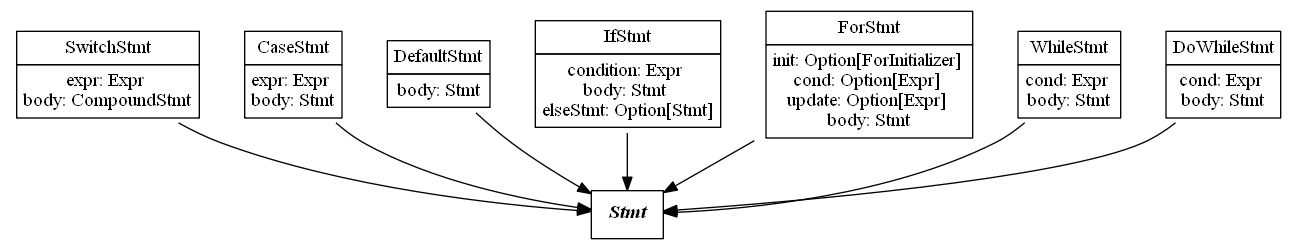
\includegraphics[scale=0.4]{data/flow_control_Stmt_classes.png}
~\\~\\Figure II.4 - Flow-control structures
\end{center}

\begin{center}
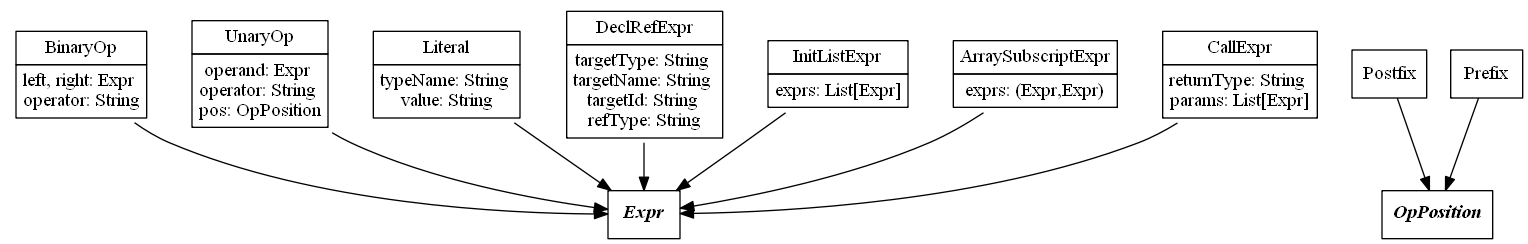
\includegraphics[scale=0.35]{data/Expr_classes.png}
~\\~\\Figure II.5 - Detail of the Expr class hierarchy
\end{center}

\paragraph{}
\hspace{4mm}\textnormal{Note that our model does not strictly represents a C++ code. For example, we do not prevent a \textit{if} to contain the instruction \textit{break}
(among other inaccuracies ...). We felt that this kind of refinement would unnecessarily complicate the task without adding anything more to the CFG analysis. 
Since the code is already semantically checked by the Clang compiler and given our future needs, we thought it would be wiser to aim for a simple model.}

\subsubsection{Important notes}

\vspace{1.5mm}
\begin{itemize}
\item To accurately represent the CFG of our input programs, we should take into account the fail-fast mechanism in the evaluation of boolean conjunctions/disjunctions.
The importance of this mechanism for our project is illustrated in the figure below.\vspace{1mm}
\item However, since the evaluation's order of the expressions is not completely specified specified in C++ (unlike Java which evaluates from left to right),
we will ignore that even if it will surely change the result for certain kind of treatments when some expressions contain side-effect sub-expressions
 (increment, assignments...).\vspace{1mm}
\end{itemize}

\begin{center}
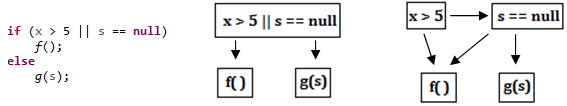
\includegraphics[scale=0.85]{data/fail-fast.png}
~\\~\\Figure II.6 - On the left the considerate code. On the center, we didn't take into account the fail-fast for the CFG, and finally on the right we consider the fail-fast
\end{center}

\paragraph{}
\hspace{4mm}\textnormal{Just to see what we are losing by ignoring that kind of things is illustrated in the figure above : if we try to
assert the property \textit {<< variable s is always initialized when g(s) is called >>}, the first CFG will not allow us to conclude
(or it will conclude \textbf {true}, erroneously) while the second allows us
to state that there are executions, according to the value of x,
where $g$ is called with an uninitialized parameter
(assuming that the left son is always a successful test and the right son is a failed test). It is not really a problem, as
we could argue that it is fine to use fail-fast most of the times but that it is safer not to use it for a critical program.}

\paragraph{}
\hspace{4mm}\textnormal{Finally, we chose to make all the classes as case-classes to enable the powerful Scala pattern-matching.
Most algorithms are recursive, the parsing of the AST being the only exception.}

\section{SourceCodeNode to CFG}

\paragraph{}
\hspace{4mm}\textnormal{Considering that Stmt and Decl children classes were partly low-level elements of the code that are not important
in the CFG, we decided to perform a last step of transformation from SourceCodeNode to ProgramNode, which is a simpler and higher level abstraction of the code.
The ProgramNode objects will be the values of the nodes of the actual graph, represented by the class GraphNode[T].}

\paragraph{}
\hspace{4mm}\textnormal{GraphNode is actually a generic type, completely independent of all the classes we introduced so far.
It basically represents any oriented unweighted graph. The conversion from SourceCodeNode to
ProgramNode is handled on the fly while constructing the CFG (GraphNode[ProgramNode]), which
consists in creating the links between the various nodes of the graph.}

\begin{center}
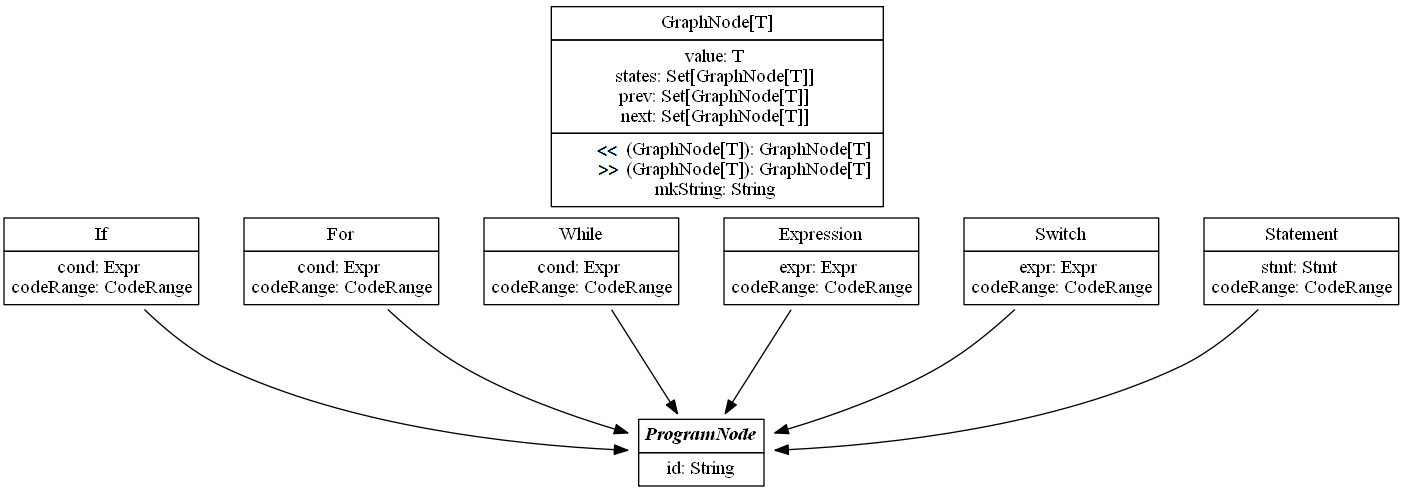
\includegraphics[scale=0.5]{data/CFG_classes.png}
~\\~\\Figure II.7 - ProgramNode class hierarchy and GraphNode
\end{center}

\paragraph{}
\hspace{4mm}\textnormal{}

\chapter{Model checking}

\section{Representation of the environments}

\subsection{}

\section{CTL expressions}

\subsection{Defining the CTL-V language}

\subsection{Evaluation of the predicates}

\end{document}
